\chapter{Mini-KaZaA Client}
Oltre che di un Bootstrap server, la rete Mini-KaZaA si basa su un client che gli utenti possono usare per accedere alla rete e poter condividere e scaricare file.
\section{Mini-KaZaA Client in generale}
Mini-KaZaA client presenta tutte le funzionalità che consentono una condivisione peer to peer dei contenuti.
Ogni client al primo avvio chiede all'utente, tramite un comodo pannello, di scegliere il \emph{ruolo} da interpretare all'interno della rete.

Chi ha più risorse da mettere a disposizione e una banda di comunicazione più ampia può scegliere di essere un Super Node, il quale oltre a condividere e scaricare, ha la funzione di smistare le query nella rete e accettare richieste direttamente dagli Ordinary Node \emph{figli}. Chi ha meno risorse da mettere a disposizione può scegliere di essere un semplice Ordinary Node.

\section{Il codice di Mini-KaZaA client}
Il codice di Mini-KaZaA client è distribuito in tre diverse librerie:
\begin{itemize}
 \item \textbf{lpr.minikazaa.minikazaaclient}: questa libreria contiene classi comuni a tutti e due i tipi di client dal punto di vista logico. L'esempio più evidente è la classe \verb|MainGui.java|.
 \item \textbf{lpr.minikazaa.minikazaaclient.ordinarynode}: questa libreria contiene le classi che logicamente appartengono al tipo di client Ordinary Node, ma che, all'occorrenza, possono essere importate anche da un Super Node.
 \item \textbf{lpr.minikazaa.minikazaaclent.supernode}: questa libreria, infine contiene tutte le classi che servono ad un supernodo per funzionare e che appartengono a questo logicamente. Alcune di queste classi, come per esempio \verb|SupernodeCallbacksInterface.java|, vengono utilizzate anche dagli Ordinary Node.
\end{itemize}

Questa suddivisione è puramente logica visto che i due tipi di client differiscono solo per alcune caratteristiche.

Si è preferito dividere anche le classi che contengono gli stessi task per i SN e per gli ON per poter meglio gestire il codice e renderlo più modulare.
Un esempio è rappresentato dalle classi \verb|OrdinarynodeWorkingThread.java| e \verb|SupernodeWorkingThread.java| che hanno lo stesso compito, ma, che piuttosto che complicare con una serie di 
\begin{verbatim}
if <condizione> then 
	<blocco> 
else 
	<blocco>|
\end{verbatim}
si è preferito separare in due classi distinte.

Passiamo ora a una presentazione più dettagliata del codice comune a Super Node e Ordinary Node.

\section{Le strutture dati comuni}
Per lo sviluppo di Mini-KaZaA è stato necessario predisporre una serie di strutture dati che tutto il software
utilizzi per condividere informazioni.

All'interno del package \verb|lpr.minikazaa.minikazaaclient| troviamo le seguenti classi che rappresentano strutture dati comuni a SN e ON:
\begin{itemize}
 \item \verb|NodeConfig.java|
 \item \verb|Query.java|
 \item \verb|Answer.java|
 \item \verb|SearchField.java|
 \item \verb|Download.java|
 \item \verb|DownloadRequest.java|
 \item \verb|DownloadResponse.java|
\end{itemize}

Guardiamo cosa si nasconde all'interno di ognuna delle classi sopracitate.

\subsection{NodeConfig.java}
La classe \verb|NodeConfig.java| contiene i seguenti attributi:
\newline
\begin{lstlisting}
private String user_name;
private int port;
private String bootstrap_address;
private int max_conn;
private int ttl;
private boolean is_sn;

//Calcolato all'avvio
private String my_address;
\end{lstlisting}

Questi attributi sono i campi che l'utente inserisce nel form al primo avvio del programma e contengono le informazioni di configurazione del nodo. 

\subsection{Query.java}\label{sec:query}
La classe \verb|Query.java| viene utilizzata dal client Mini-KaZaA per l'invio di richieste di file nella rete.

Contiene diversi attributi per i quali sono disponibili i metodi \verb|set| e \verb|get|. Questa classe inoltre implementa
le interfacce \verb|Serializable| e \verb|Cloneable|.
La prima serve per poter inviare su rete come flusso di byte l'oggetto \verb|Query|. La seconda invece serve per poter
copiare un'istanza dell'oggetto \verb|Query| in una seconda istanza.
\newline
\begin{lstlisting}
//Espressione regolare della query
private String body_q;

//Query di risposta
private Answer body_a;

//Sorgente di una query
private NodeInfo id_origin;

//NodeInfo del mittente
private NodeInfo sender;

//NodeInfo del destinatario
private NodeInfo receiver;

//Time to live della query
private int ttl;

//Id della query attribuito dall'origine
private int id;
\end{lstlisting}

La classe \verb|Query| ha tre gruppi di attributi.Un primo gruppo descrive il contenuto della query e di conseguenza
il tipo di query. Un secondo gruppo serve per identificare i soggetti coinvolti nello scambio della query stessa.
Il terzo gruppo contiene invece parametri per l'identificazione della query. 

Analizziamo uno ad uno questi parametri per capire meglio come funzionano le query in Mini-KaZaA.
\begin{itemize}
 \item \verb|body_q|:
il vero corpo della query di richiesta di un file. \`{E} una stringa che contiene un
espressione regolare che il client Mini-KaZaA riesce a interpretare;

 \item \verb|body_a|:
la parte dell'oggetto \verb|Query| che contiene la risposta a una determinata richiesta. Analizzaremo la classe
\verb|Answer| successivamente;

 \item \verb|id_origin|:
per ogni query deve essere nota l'origine dalla quale proviene la query stessa per poi poterla correttamente fermare
al punto giusto e farla ritornare al mittente. Questo è il compito del campo \verb|id_origin|;

 \item \verb|sender|: 
questo campo indica uno dei due soggetti che sono impegnati in un singolo scambio di query, il nodo da cui parte;

 \item \verb|receiver|:
questo campo indica il nodo a cui deve arrivare la query in uno scambio;

 \item \verb|ttl|:
questo campo sta per \emph{Time To Live} e indica il numero di scambi per il quale la query deve continuare a esistere.
Serve principalmente per evitare che si creino dei cicli infiniti di scambio della query ottenendo quindi una valanga
di dati ridondanti con conseguente intasamento della rete;

 \item \verb|id|:
ogni nodo può inviare più query alla volta nella rete e il compito di questo campo è di identificare univocamente la
query presso il suo nodo origine.
\end{itemize}

\subsection{Answer.java}
La classe \verb|Answer.java| contiene i file che possono corrispondere ai criteri di una ricerca. 

\`{E} una classe molto semplice ma molto utile per indicizzare rapidamente i file.

Ecco il codice nel quale vengono dichiarati gli attributi della classe.
\newline
\begin{lstlisting}
//File che corrispondono a una query
private ArrayList <OrdinarynodeFiles> files;

//Id della query assegnato dall'origine
private int id;
\end{lstlisting}

L'attributo \verb|files| è una lista di OrdinarynodeFiles, Sezione \ref{sec:on_files}.

L'attributo \verb|id| richiama semplicemente l'id univoco della query di cui fa parte l'oggetto \verb|Answer|.

\subsection{SearchField.java}\label{sec:searchField_class}
La classe \verb|SearchField.java| viene utilizzata dal client Mini-KaZaA per tenere in memoria tutti i risultati
associati a una richesta di file.
Da uno di questi campi poi vengono estratte le informazioni per eventuali download di file.

Anche questa classe è piuttosto semplice poichè funziona da appoggio alla rappresentazione grafica e per snellire
la quantità di informazioni da tenere in memoria per l'utente.

Il codice che descrive gli attributi della classe è il seguente:
\newline
\begin{lstlisting}
//File owner
private NodeInfo owner;

//File descriptor
private MKFileDescriptor file;
\end{lstlisting}

Con queste due semplici informazioni è possibile sia risalire al proprietario, compreso l'indirizzo ip da contattare
per il download, sia ottenere tutti i metadati\footnote{Quando parliamo di metadati ci riferiamo alle informazioni che riguardano i file, come la dimensione, il path assoluto ecc. Queste informazioni si possono sempre ricavare perchè salvate all'interno del file.} del file da scaricare\footnote{I download così come le ricerche vengono
effettuati mediante l'hash univoco md5 che tratteremo nella Sezione \ref{sec:md5}}.

\subsection{Download.java}\label{sec:download_class}
La classe \verb|Download.java| serve al client Mini-KaZaA per indicizzare i downloads che si effettuano. Questa classe si distingue da \verb|SearchField.java| perchè mantiene anche il numero di byte già scaricati.
\newline
\begin{lstlisting}
private MKFileDescriptor file_to_download;
private long downloaded_bytes;
private String downloader_path;

public Download(MKFileDescriptor file){

	this.file_to_download = file;
	this.downloaded_bytes = 0;

	//Directory di default
	this.downloader_path = "./downloads/";
}
\end{lstlisting}

Gli attributi della classe \verb|Download.java| sono quelli elencati nel listato mostrato appena sopra.
\verb|file_to_download| identifica il file che si sta scaricando tramite il codice hash \emph{md5}. Viene anche usato il nome del file, salvato all'interno di \verb|MKFileDescriptor|, per poter comporre il path assoluto con l'attributo \verb|downloader_path|. I \verb|downloaded_bytes| invece indicano, quanta parte di file è stata già scaricata dalla rete.

\subsection{DownloadRequest.java}
La classe \verb|DownloadRequest.java| viene utilizzata dal client Mini-KaZaA per richiedere file da scaricare al nodo che lo possiede.
Si compone dei seguenti attributi:
\newline
\begin{lstlisting}
//File da scaricare
private String file_request;

//Sorgente della richiesta
private NodeInfo request_source;
\end{lstlisting}

\subsection{DownloadResponse.java}
Il client Mini-KaZaA fa un uso particolare della classe \verb|DownloadResponse.java|. Essa viene infatti usata sia per inizializzare e terminare una comunicazione, sia come ``mezzo di trasporto'' delle varie parti di un file.

Vediamo innanzitutto quali attributi include questa classe:
\newline
\begin{lstlisting}
//byte che compongono una parte di 
//un file
private byte [] part;

//File inviato
private String file;
\end{lstlisting}
Mini-KaZaA ``spezzetta'' il file da inviare in piccoli pacchetti da 4Kb che vengono inseriti all'interno dell'array \verb|part|.
\verb|file| invece contiene l'md5 del file che viene inviato. Questa classe, e la combinazione dei suoi paramtri, permettono a Mini-KaZaA di controllare l'inizio di una comunicazione, la fine della stessa, e tutti gli invii intermedi di byte.
Vedremo meglio come funziona lo scambio di file all'interno della Sezione \ref{sec:scambio}

\section{Il percorso di una query}
Nella sezione \ref{sec:query} abbiamo visto di cosa si compone la classe \verb|Query.java|. Ora vediamo come viene utilizzata dal client nello scambio di richieste.

Ogni query di ricerca di file comincia con l'input dell'utente tramite un apposita form di cui parleremo nella Sezione \ref{sec:grafica}.
Viene così generato un oggetto di tipo query con il seguente frammento di codice:
\begin{lstlisting}
Query q = new Query();
q.setId(this.my_num);
q.setSender(this.my_infos);
q.setOrigin(this.my_infos);
q.setAskingQuery(this.search_tf.getText());
q.setTTL(this.my_conf.getTimeToLeave());
\end{lstlisting}
Questo oggetto viene così inviato nella rete attraverso i SN.
Ogni SN leva un'unità di \emph{TTL} alla query e la rimbalza nella rete.

La gestione del percorso di una query è affidata completamente alla classe \verb|SupernodeTCPWorkingThread.java| e ne parleremo in Sezione \ref{sec:smistamento_delle_query}.
Quest'operazione è comune ai due tipi di client, ma contiene delle ovvie differeze, dovute alla natura dei vari nodi, che spiegheremo più avanti.

\section{La classe SupernodeList.java}
La classe \verb|SupernodeList.java| è una delle classi principali del progetto. Essa infatti mantiene un elenco dei SN presenti sulla rete.
Essa in realtà è molto utile per indicizzare insiemi di nodi di qualsiasi tipo, difatti il Bootstrap server utilizza proprio questa classe per le sue liste di nodi.

Come si può vedere dal seguente listato:
\begin{lstlisting}
private ArrayList<NodeInfo> sn_list;
private ArrayList<NodeInfo> sub_set_list;

public SupernodeList() {
	this.sn_list = new ArrayList();
	this.sub_set_list = null;
}
\end{lstlisting}

la classe \verb|SupernodeList.java| è composta da due attributi:
\begin{itemize}
 \item \verb|sn_list|:
un'\emph{ArrayList} di \verb|NodeInfo| utilizzata per tenere in memoria \emph{tutti} i nodi della rete;

 \item \verb|sub_set|:
una seconda \emph{ArrayList} di \verb|NodeInfo| utilizzata di volta in volta per memorizzare un sottoinsieme di nodi vicini e convenienti da contattare.
\end{itemize}

La classe fornisce anche tutti i metodi per gestire al meglio l'elenco di nodi.

Per prima cosa ci sono due overload per quanto riguarda il calcolo della latenza di un nodo\footnote{La latenza viene calcolata in ms tramite una procedura che prende il nome di \emph{ping} che vedremo in Sezione \ref{sec:ping}}

Il metodo in questo listato
\begin{lstlisting}
public synchronized void 
refreshPing(InetAddress ia, int port, long new_ping) {
	for (NodeInfo n : sn_list) {
		//Confrontiamo l'indirizzo del nodo estratto 
		//con quello passato come parametro del metodo
		if (n.getIaNode().toString().equals(ia.toString())) {
			if (n.getDoor() == port) {
				n.setPing(new_ping);
			}
		}
	}
}
\end{lstlisting}
viene usato solo per cambiare il valore della latenza a un nodo specifico.

Il secondo overload del metodo mostrato in precedenza consente invece di effettuare una passata di tutti i nodi che abbiamo nella nostra lista e di aggiornarne il valore della latenza.
\begin{lstlisting}
public synchronized void refreshPing() {
	//Thread pool
	ThreadPoolExecutor my_thread_pool =
		new ThreadPoolExecutor(
			10, 15, 50000L, 
			TimeUnit.MILLISECONDS,
			new LinkedBlockingQueue<Runnable>());
	
	if (this.sn_list.size() >= 1) {
		for (NodeInfo n : sn_list) {
			NodePing pinging = 
				new NodePing(
					n.getIaNode(), 
					n.getDoor(), 
					this);

			my_thread_pool.execute(pinging);
		}
	}
	my_thread_pool.shutdown();

	this.setChanged();
	this.notifyObservers();
}
\end{lstlisting}
Questo metodo invece non vuole parametri poichè effettua l'aggiornamento su tutto il set di nodi.

Mini-KaZaA crea un overlay network dinamico grazie al metodo \verb|subSet()| che seleziona un insieme di SN valutati come ``vicini'', Sezione \ref{sec:ping}, a seconda della loro latenza. Per esplorare nuove porzioni della rete ne sceglie due sopra i 50ms di latenza e tutti gli altri al di sotto. Di seguito riportiamo la porzione di codice che si occupa di questa scelta.

\begin{lstlisting}
public synchronized void 
subSet(int set_size, long threshold) {
	ArrayList<NodeInfo> neighbors = new ArrayList();

	for (NodeInfo n : this.sn_list) {
		if (n.getPing() != -1) {

			if (n.getPing() <= threshold) {
				neighbors.add(n);
				if (neighbors.size() == set_size) {
					this.sub_set_list = neighbors;
				}
			}
		}
	}

	this.sub_set_list = neighbors;
}

public synchronized ArrayList<NodeInfo> getSubSet() {

	if (this.sub_set_list == null) {
		subSet(10, 100);
	}

	return this.sub_set_list;
}
\end{lstlisting}

Per gli Ordinary Node che devono scegliere il loro Super Node di rifermento la classe \verb|SupernodeList.java| mette a disposizione un metodo che seleziona il nodo ``migliore'' al quale connettersi. Il metodo si chiama \verb|getBest()| e il codice che lo riguarda è riportato di seguito.
\begin{lstlisting}
public synchronized NodeInfo getBest() {
	NodeInfo best = new NodeInfo();

	for (NodeInfo candidate : this.sn_list) {
		if (best.getIaNode() == null) {
			best.setInetAddress(candidate.getIaNode());
			best.setCallbacksInterface(
				candidate.getCallbackInterface());
			best.setDoor(candidate.getDoor());
			best.setId(candidate.getId());
			best.setUsername(candidate.getUsername());
			best.setPing(candidate.getPing());
		} else {
			if (candidate.getPing() < best.getPing()) {
				best.setInetAddress(candidate.getIaNode());
				best.setCallbacksInterface(
					candidate.getCallbackInterface());
				best.setDoor(candidate.getDoor());
				best.setId(candidate.getId());
				best.setUsername(candidate.getUsername());
				best.setPing(candidate.getPing());
			}
		}
	}
	
	return best;
}
\end{lstlisting}


\section{Il paradigma Observable-Observer}\label{sec:obs-obs}

Il linguaggio Java fornisce due classi molto utili per gestire in modo asincrono i cambiamenti di stato di determinate strutture dati.

\begin{figure}[t]
 \centering
 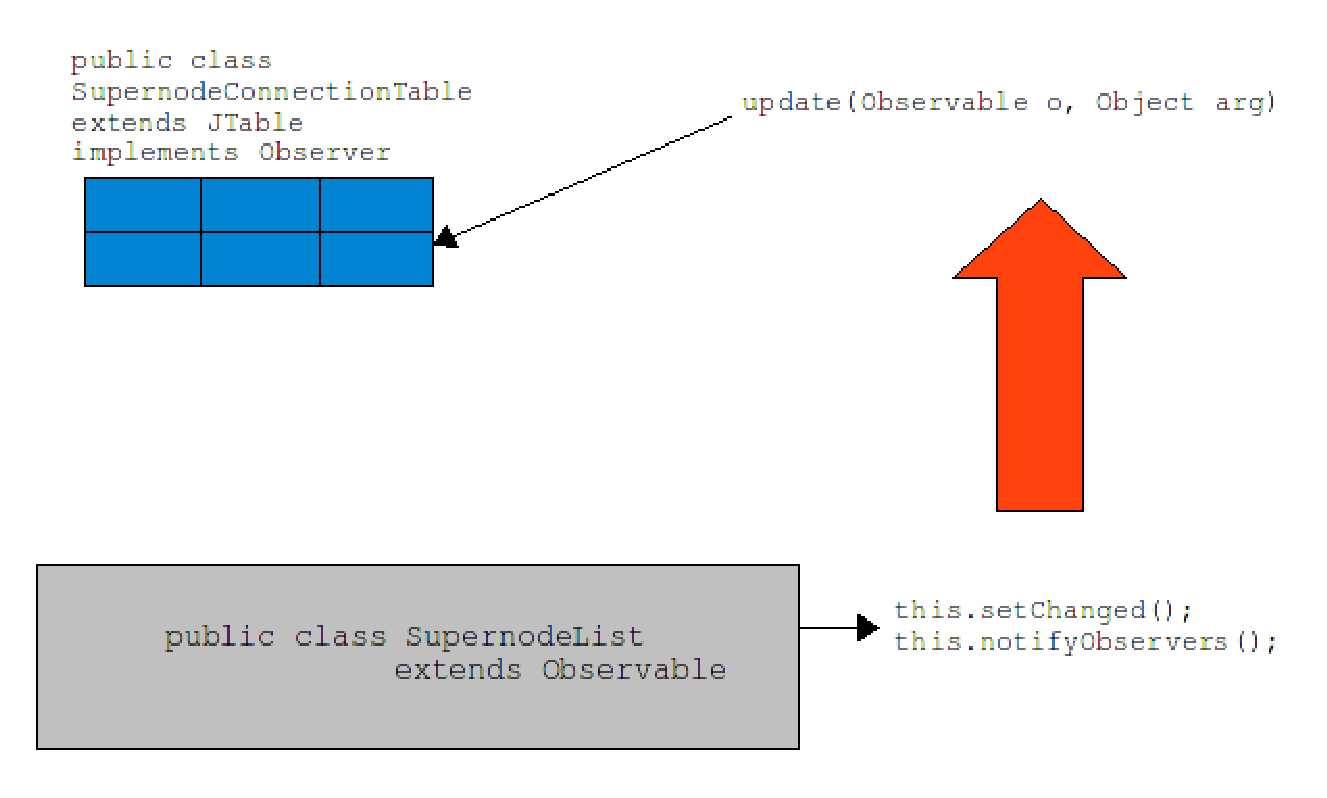
\includegraphics[width=218.72px,height=129.12px,bb=14 14 635 381]{images/observable.eps}
 % observable.eps: 0x0 pixel, 300dpi, 0.00x0.00 cm, bb=14 14 635 381
 \caption{Paradigma Observable - Observer}
 \label{fig:observable}
\end{figure}

\`{E} molto utile, infatti, avere un modo agile e integrato nel linguaggio di nodificare ogni cambiamento che subisce una struttura dati. Esempi che riguardano Mini-KaZaA sono molto frequenti: la struttura dati che memorizza i file trovati e la tabella che li deve mostrare in grafica, la lista di SN e la tabella di Net Monitor e così via.

Java mette a disposizione la classe \verb|Observable|,%extends Observable
con la quale è possibile mettere ``sotto osservazione'' una determinata classe che estende Observable con il comando \verb|public class MyClass extends Observable|, e la classe \verb|Observer|, che va implementata con il comando \verb|public class MyClass| \verb|implements Observer|.

La situazione che si viene a creare è mostrata in Figura \ref{fig:observable}.
La prima classe fornisce due metodi che vanno richiamati ogni qual volta si effettua una modifica all'oggetto che estende \verb|Observable|:
\begin{lstlisting}
this.setChanged();
this.notifyObservers();
\end{lstlisting}
Questi due metodi svegliano il metodo \verb|update()|, di cui deve essere fatto \emph{obbligatoriamente} l'override, che è contenuto nella classe che implementa \verb|Observer|.
La firma del metodo è sempre la solita:
\begin{lstlisting}
public void update(Observable o, Object arg)
\end{lstlisting}
Il primo parametro rappresenta l'oggetto che ha chiamato il metodo \verb|update()|. Per generalizzare il metodo,
questo parametro rappresenta un \emph{Observable} sul quale poi dovrà essere fatto un'operazione di \emph{cast}
per convertirlo nell'oggetto corretto e poter utilizzare le sue funzioni. Il secondo parametro rappresenta i parametri aggiuntivi che possono essere utili al metodo update.
Il metodo update definirà quindi tutte le operazioni che dovranno essere fatte a ogni aggiornamento della struttura dati sotto osservazione.

\section{Ping dei nodi}\label{sec:ping}
Ogni client Mini-KaZaA ha bisogno di sapere quanto dista dalla rete e, di conseguenza, quanto i nodi della rete distano da lui.
Come unità di misura per la distanza da un nodo all'altro vengono usati i millisecondi che intercorrono dall'invio di un particolare pacchetto alla ricezione del pacchetto di risposta.

In Mini-KaZaA sono stati implementati due \emph{Task}: NodePing e NodePong.
Il primo task crea un pacchetto Datagram con le seguenti istruzioni:
\begin{lstlisting}
DatagramSocket my_datagram_socket = null;

try {
	my_datagram_socket = new DatagramSocket();
} catch (SocketException ex) {
	//Log
}
		
byte [] data = new byte[32];

DatagramPacket pack = 
new DatagramPacket(
	data,
	data.length, 
	host_ia, 
	host_port);

//Preparazione del pacchetto package
pack.setData(data,0,data.length);
pack.setLength(data.length);
\end{lstlisting}
dopo di che lo invia al nodo destinatario e fa partire un timer.
\begin{lstlisting}
long start_time = System.currentTimeMillis();

try {
	my_datagram_socket.send(pack);
} catch (IOException ex) {
	//Log
}
\end{lstlisting}
Non appena arriva il medesimo pacchetto di risposta viene calcolato il tempo in millisecondi intercorsi fra l'invio e la ricezione del pacchetto e questa sarà la stima della distanza fra i due nodi.
Le istruzioni che si occupano della ricezione del pacchetto sono le seguenti:
\begin{lstlisting}
try {

	my_datagram_socket.receive(pack);
} catch (IOException ex) {
	//Log
}

long arrive_time = System.currentTimeMillis();

long ping = arrive_time - start_time;
\end{lstlisting}
Il secondo task invece funziona con il procedimento opposto. Ovvero, inizialmente predispone un socket di ascolto sulla porta scelta dall'utente al primo avvio del programma.
\begin{lstlisting}
int port = this.my_conf.getPort();
DatagramSocket pong_sock = null;
try {
	pong_sock = new DatagramSocket(port);
} catch (SocketException ex) {
	//Log
}
\end{lstlisting}
Poi entra in un ciclo infinito, che verrà interrotto solo dall'uscita del programma, il cui unico compito è quello di rispondere il più velocemente possibile alle richieste di ``ping'' che arrivano alla porta del socket.

\begin{lstlisting}
while (true) {

	byte[] packet = new byte[32];

	DatagramPacket pack = 
		new DatagramPacket(
			packet, 
			packet.length);

	try {

		pong_sock.receive(pack);
	} catch (IOException ex) {
		//Log
	}
	packet = pack.getData();
	DatagramSocket send_sock = null;
	try {

		send_sock = new DatagramSocket();
	} catch (SocketException ex) {
		//Log
	}

	byte [] send_byte = packet;
	DatagramPacket send_pack = 
		new DatagramPacket(
			send_byte,
			send_byte.length,
			pack.getAddress(),
			pack.getPort());

	try {

		send_sock.send(send_pack);
	} catch (IOException ex) {
		//Log
	}
	
}
\end{lstlisting}
Ovviamente ogni errore o eccezione che è sollevata in questi frammenti di codice viene loggata per future analisi\footnote{In questi frammenti di codice abbiamo omesso la chiamata allaclasse di log per concentraci maggiormente sulle istruzioni che sono più strettamente legate alle misurazioni delle latenze tramite socket UDP}

\section{Invio di file e divisione del file in parti.}\label{sec:download_tcp}\label{sec:scambio}
L'attività principale che Mini-KaZaA prevede è lo scambio di file. I file vengono trasmessi sulla rete, anche su grandi distanze.
I file possono anche essere molto grandi quindi non conviene inviare tutto il file in un unico momento. \`{E} molto più conveniente dividere il file in parti.
Di questo si occupa la parte che invia il file nel \emph{TCPWorkingThread}.
Il codice che esegue queste operazioni è comune a tutti i tipi di nodi, dato che sia SN che ON possono inviare file sulla rete, ed è esposto nel seguente listato.
\begin{lstlisting}
if (incoming_obj instanceof DownloadRequest) {
	//Devo spedire il file richiesto
	DownloadRequest request = 
		(DownloadRequest) incoming_obj;

	MKFileDescriptor file_to_send = 
		this.my_files.getFileList(request.getFile());

	Socket send_sock = new Socket(
			request.getSource().getIaNode(),
			request.getSource().getDoor());

	ObjectOutputStream output = 
		new ObjectOutputStream
		(send_sock.getOutputStream());

	//Avvisa l'inizio del trasferimento.
	DownloadResponse init_response = 
		new DownloadResponse(null, file_to_send.getMd5());

	output.writeObject(init_response);

	File file_pointer = new File(file_to_send.getPath());

	FileInputStream in_file = 
		new FileInputStream(file_pointer);

	byte[] buffer = new byte[4096];

	while (true) {
		try {
			int letti = in_file.read(buffer);
			if (letti > 0) {
				DownloadResponse filepart = 
					new DownloadResponse(buffer, null);
				output.writeObject(filepart);
			} else {
				break;
			}
		} catch (IOException e) {
			break;
		}
	}

	//Chiude la comunicazione
	DownloadResponse stop_sending = 
		new DownloadResponse(null, file_to_send.getMd5());
	output.writeObject(stop_sending);

	in_file.close();
	output.flush();
	output.close();

	send_sock.close();

	
}
\end{lstlisting}
Il procedimento è standard. Ovvero, prima si inizializza la connessione con una prima comunicazione, poi si inviano le varie parti di file e infine si chiude la comunicazione.

Dall'altro lato si troverà chi ha inviato la richiesta di download e che ora si prepara alla ricezione.
Il listato che riceve il file è il duale di quanto appena mostrato ed è il seguente.
\begin{lstlisting}
if (incoming_obj instanceof DownloadResponse){
	DownloadResponse response = 
		(DownloadResponse) incoming_obj;

	//Inizio dell'invio di un file.
	if (response.getPart() == null) {
		Download file_dl = 
			this.my_dl_monitor.getDownload(response.getFile());
		
		File file = new File(
			file_dl.getDownloaderPath() + 
			file_dl.getFile().getFileName());
		
		FileOutputStream file_downloading = 
			new FileOutputStream(file);
		
		while (true) {
			Object read_part = input_object.readObject();

			if (read_part instanceof DownloadResponse) {
				DownloadResponse part = (DownloadResponse) read_part;
				if (part.getFile() == null) {
					//Posso inserire la parte sia 
					//nel monitor che nel file effettivo.
					byte[] buffer = part.getPart();

					if (buffer.length > 0) {
						file_downloading.write(buffer, 0, buffer.length);
						part.setFile(file_dl.getFile().getMd5());
						this.my_dl_monitor.addBytes(part);
					}
				}
				else{
					break;
				}
			}
		}

		file_downloading.flush();
		file_downloading.close();
	}
\end{lstlisting}

\section{La grafica del client Mini-KaZaA}\label{sec:grafica}
\begin{figure}[t]
 \centering
 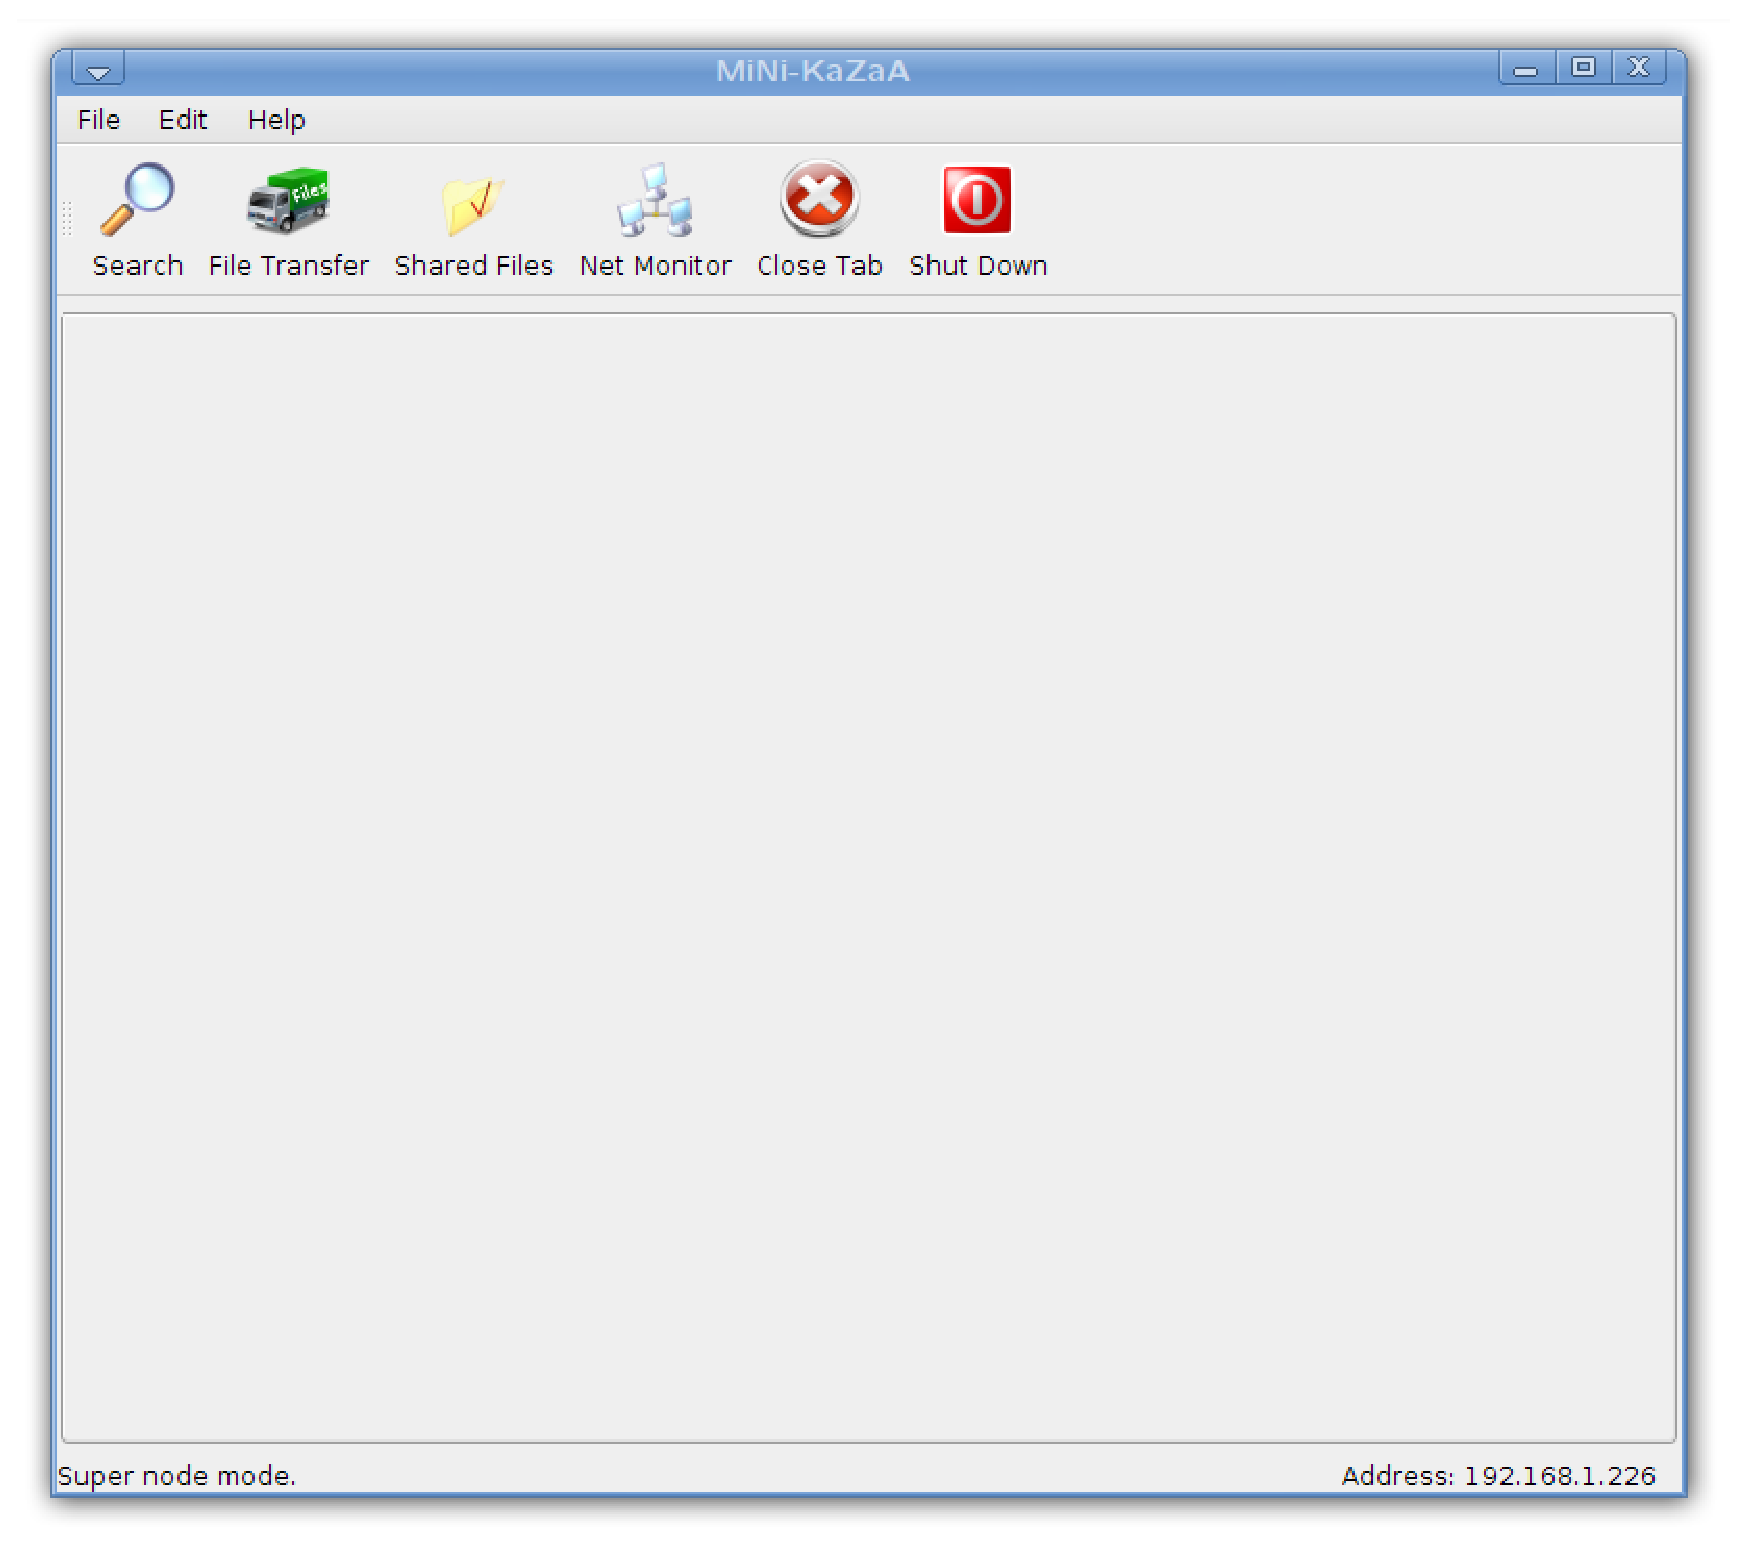
\includegraphics[width=270px,height=245px,bb=14 14 841 737]{images/mini_kazaa_client.eps}
 % mini_kazaa_client.eps: 0x0 pixel, 300dpi, 0.00x0.00 cm, bb=14 14 841 737
 \caption{L'interfaccia grafica principale del client.}
 \label{fig:mini_kazaa_client}
\end{figure}
Il client Mini-KaZaA è dotato di un front-end grafico per facilitarne l'utilizzo agli utenti finali. La grafica di Mini-KaZaA è scritta usando le librerie Swing, che mette a disposizione il linguaggio Java, con un unica differenza:
\begin{lstlisting}
try {
	UIManager.setLookAndFeel(UIManager.getSystemLookAndFeelClassName());
} catch (Exception ex) {
}
\end{lstlisting}
con queste operazioni si vuole che la grafica Swing ottenga il rendering dall'environment di sistema. Questo comando funziona, per il momento, solamente in ambiente grafico Win e Gnome (GTK+2), mentre non viene attivato, e quindi vengono visualizzati con il rendering originale i componenti Swing, su KDE\footnote{Sistemi utilizzati per questo tipo di test: Windows Vista(Win), Ubuntu(Gnome), Xandros OS (KDE).}

L'interfaccia principale (Figura \ref{fig:mini_kazaa_client}), comune a tutti i tipi di nodi si divide in quattro parti principali:
\begin{enumerate}
 \item \textbf{Barra dei menù:}
la prima barra in alto dove è possibile trovare il menù:
	\begin{enumerate}
		\item \textit{File}: per le operazioni sul client;
		\item \textit{Edit}: per il controllo delle configurazioni;
		\item \textit{Help}: per ottenere aiuto e informazioni su Mini-KaZaA.
	\end{enumerate}

 \item \textbf{Barra dei pannelli:}
contiene dei grossi pulsanti che attivano dei pannelli per le varie operazioni;

 \item \textbf{Panel Box:}
il riquadro centrale nel quale compaiono e scompaiono i vari pannelli attivabili dalla barra;

 \item \textbf{Barra di stato:}
posizionata in fondo alla finestra contiene informazioni di sistema riguardante il client Mini-KaZaA.
\end{enumerate}

Nella \emph{barra dei pannelli} troviamo sei pulsanti, ognuno dei quali ha una precisa funzione:
\begin{enumerate}
 \item \textbf{Search:} apre un pannello per la ricerca dei file nella rete;
 \item \textbf{File transfer:} apre un pannello che consente di monitorare lo stato dei download in corso;
 \item \textbf{Shared Files:} apre un pannello nel quale è possibile aggiungere o rimuovere file da condividere nella rete;
 \item \textbf{Net Monitor:} se si è un SN questo pulsante è abilitato e consente di vedere quali super nodi ci sono nella rete, mentre se si è un ON non sarà possibile utilizzarlo;
 \item \textbf{Close Tab:} ogni nuovo pannello viene aperto in un \emph{tab} a se stante, per questo tramite questo bottone sarà possibile chiudere i \emph{tab} aperti;
 \item \textbf{Shut Down:} consente di chiudere il programma.
\end{enumerate}



